%%
% The BIThesis Template for Bachelor Graduation Thesis
%
% 北京理工大学毕业设计开题报告 —— 使用 XeLaTeX 编译
%
% Copyright 2020 Spencer Woo
%
% This work may be distributed and/or modified under the
% conditions of the LaTeX Project Public License, either version 1.3
% of this license or (at your option) any later version.
% The latest version of this license is in
%   http://www.latex-project.org/lppl.txt
% and version 1.3 or later is part of all distributions of LaTeX
% version 2005/12/01 or later.
%
% This work has the LPPL maintenance status `maintained'.
%
% The Current Maintainer of this work is Spencer Woo.
%
% This work consists of the files main.tex, misc/cover.tex and
% the external PDF misc/reviewTable.pdf
%
% Compile with: xelatex -> biber -> xelatex -> xelatex
\documentclass[proposal-report]{bitart}
\usepackage{float}
\usepackage{listings}
\usepackage{fontspec}
\usepackage{xcolor}
\setmonofont{Consolas}
\usepackage{algorithm}
\usepackage{algpseudocode}
\usepackage{amsmath}
\usepackage[hidelinks]{hyperref}
\renewcommand{\algorithmicrequire}{\textbf{Input:}}
\renewcommand{\algorithmicensure}{\textbf{Output:}}



\lstset{
basicstyle=\small,%
escapeinside=``,%
keywordstyle=\color{red} \bfseries,% \underbar,%
identifierstyle={},%
commentstyle=\color{blue},%
stringstyle=\ttfamily,%
%labelstyle=\tiny,%
extendedchars=false,%
linewidth=\textwidth,%
numbers=left,%
numberstyle=\tiny \color{blue},%
frame=trbl%
}

% 参考文献引用文件 refs.bib
\addbibresource{misc/refs.bib}


\newcommand{\deptName}{计算机学院}
\newcommand{\majorName}{计算机科学与技术}
\newcommand{\className}{0711802}
\newcommand{\yourName}{田佳析}
\newcommand{\mentorName}{李元章}
\newcommand{\offCampusMentorName}{无}

% 定义一个概念
\newtheorem{definition}{概念}[section]



%%
% 文档开始
\begin{document}
% 评审表
% 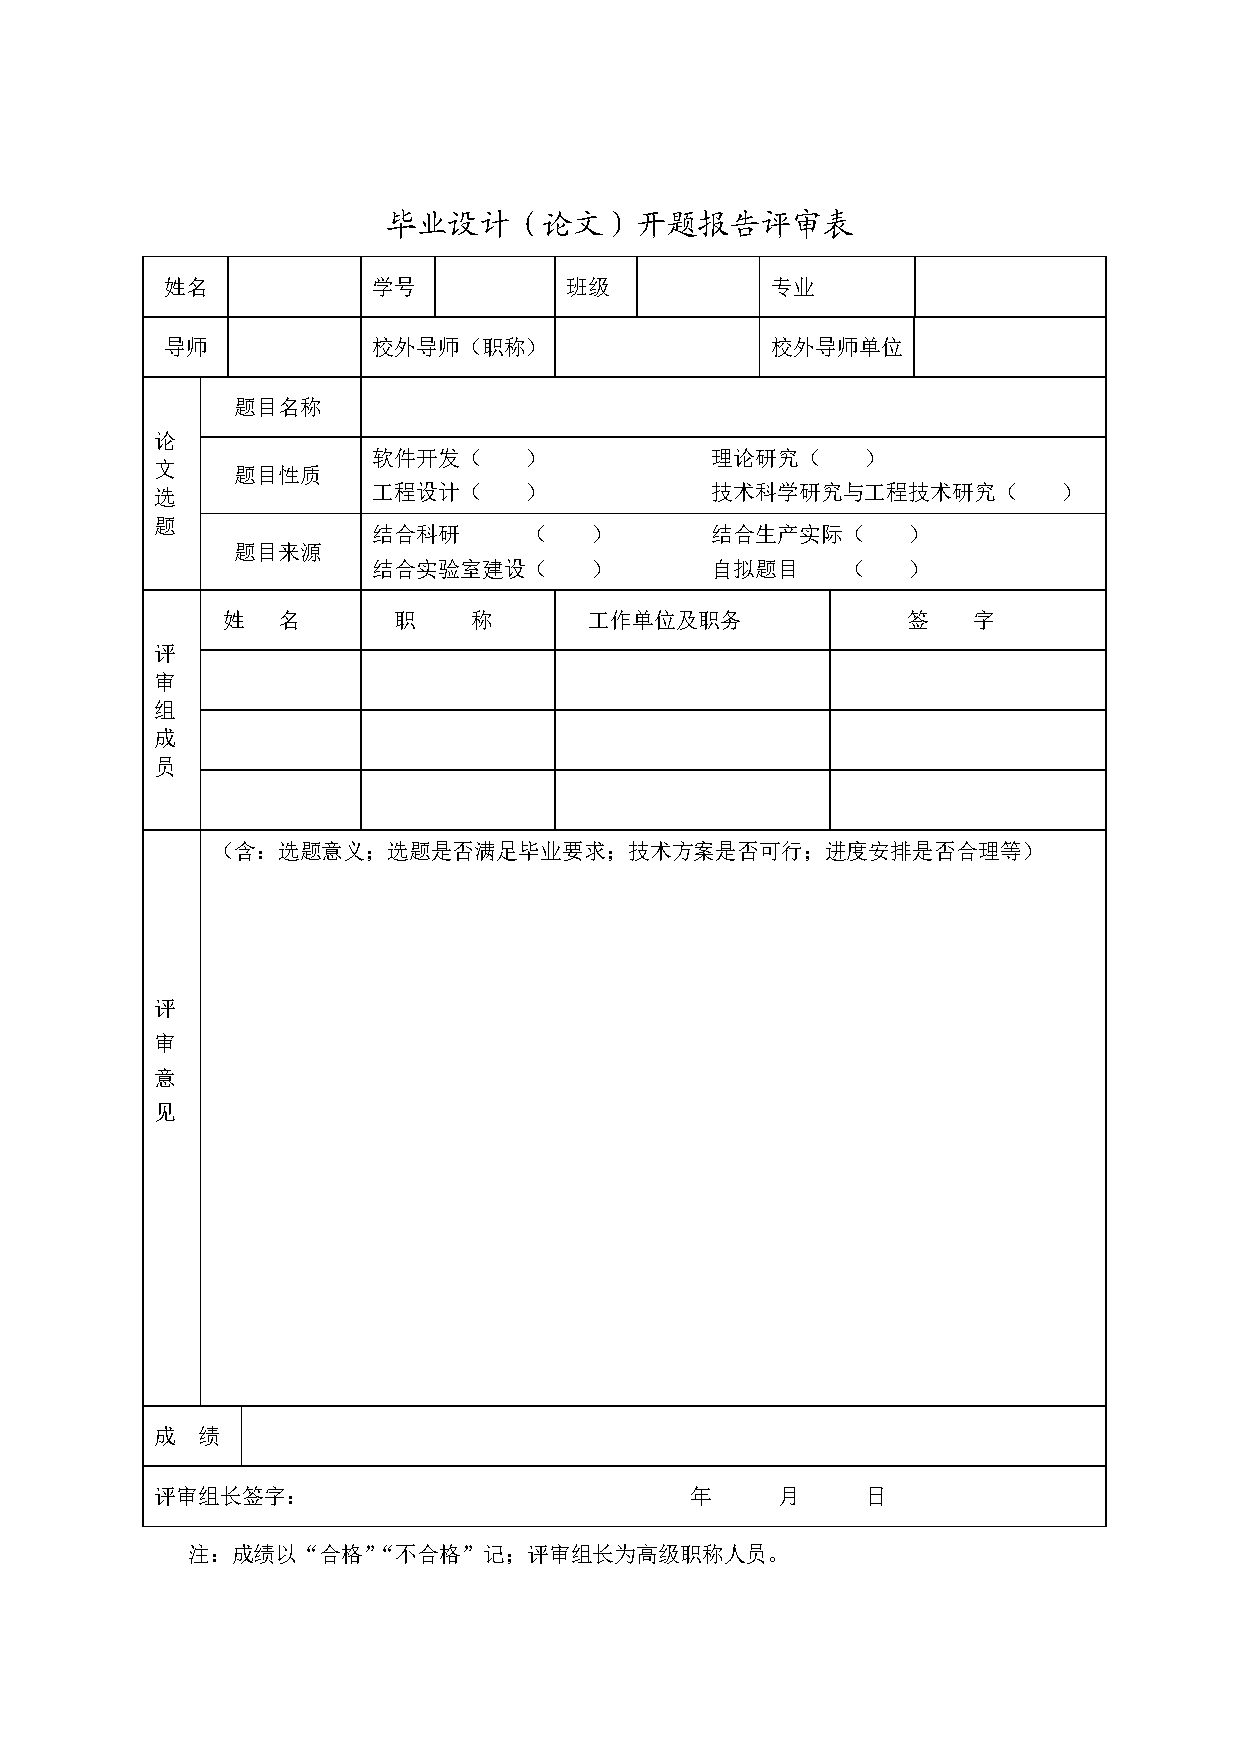
\includepdf[pages=-]{misc/reviewTableBlank.pdf}

%%
% 正文开始
\pagestyle{fancy}
% 正文从第一页开始计算页码
\setcounter{page}{1}


% 正文 22 磅的行距,段前段后间距为 0
\setlength{\parskip}{0em}
\renewcommand{\baselinestretch}{1.53}
% 正文首行悬挂 1.02cm
\setlength{\parindent}{1.02cm}

\tableofcontents
\newpage

% 内容开始


\section{实验介绍}

在五个编程实验中,我选择了大数相乘、文件比较和计算器实验,通过大数相乘实验,我学会使用汇编语言实现控制台的功能;通过文件比较,我学会了使用 win32 api 函数构建窗口;结合前面两个实验了解到的指示,我实现了一个功能较为全面的窗口计算器程序。

\section{大数相乘}

\subsection{实验要求}

要求实现两个十进制大整数的相乘(100位以上),输出乘法运算的结果。

\subsection{实验内容}

大数乘法在读入数据后,使用 fft 变换计算两个大数的乘积。

\subsection{实验过程}

整个程序过程为,将输入的数字存储转化为浮点数存储在数组中,接下来对输入的数进行 fft 变换,得到点值表示的数后两数相乘,进行 fft 逆变换,最后对逆变换得到的结果进行处理并输出。

\subsubsection{输入处理}

对于输入的数字,需要经过翻转数字,将数字每一位转换位复数形式以便利用 fft 的多项式快速乘法计算乘积,然后需要计算乘积达到的最大位数,将复数数组拓展到大于该位数的 2的幂次位,便于 fft 二分计算。

由于乘积结果位数可能大于乘数,所以为了便于位数扩展,将低位数放在数组前面,高位数放在数组后面,这时需要翻转数字,首先需要获取输入数字长度:

\begin{lstlisting}[language={[x86masm]Assembler}]
  mov esi, str_p
  mov ecx, 0
  main_loop:
      mov eax, [esi]
      cmp eax, 0
      jz loop_end
      inc ecx
      inc esi
      jmp main_loop
  loop_end:
\end{lstlisting}

遍历输入的数组,如果识别到末尾 0,ecx 保存数组长度, 跳出循环进行数组的翻转:

\begin{lstlisting}[language={[x86masm]Assembler}]
  mov esi, str_p
  mov ebx, 0
  loop1:
      mov al, [esi+ebx]
      mov dl, [esi+ecx-1]
      mov [esi+ecx-1], al
      mov [esi+ebx], dl
      inc ebx
      dec ecx
      cmp ecx, ebx
      jle loop1_end
      jmp loop1
  loop1_end:
      ret
\end{lstlisting}

上面的代码中,ecx 保存数组末尾下标,ebx 保存数组开始下标,交换 ecx 和 ebx 下标的数据,当 ecx 小于等于 ebx 时跳出循环。

之后需要将输入的数字转换为复数形式,调用 changenum 函数进行数字的转换,我建立了一个结构体用于储存数据,定义如下:

\begin{lstlisting}[language={[x86masm]Assembler}]
  cp STRUCT
    x dword ? ;实部,为 float 类型
    y dword ? ;虚部,为 float 类型
  cp ENDS
\end{lstlisting}

由于 changenum 函数代码过长,所以采用伪代码说明:

% //TODO 伪代码
\makeatletter
\def\BState{\State\hskip-\ALG@thistlm}
\makeatother
\begin{algorithm}[htb]
  \caption{数字转换为复数数组}
  \begin{algorithmic}
    \Require
      数字的首地址,复数数组的首地址
    \Ensure
      复数数组的长度
    \Procedure{ASM Procedure}{}
    \State 将数字首地址赋给 esi, 复数数组首地址赋给 edi .
    \State 初始化临时变量 n,表示数组长度.
    \BState \emph{arr\_loop}:
    \State 利用 esi 遍历数字.
    \If {[esi] == 0}
    \State \textbf{goto} \emph{done}.
    \EndIf
    \If {[esi] == '-'} 
    \State \textbf{goto} \emph{negtive}.
    \EndIf
    \State 调用 int\_to\_float函数,将整数转换为浮点数表示.
    \State 将结果赋给 [edi] 的实部.
    \State inc esi.
    \State inc n.
    \State add edi, 8.
    \State \textbf{goto} \emph{arr\_loop}.
    \BState \emph{negtive}:
    \State 符号标志取反
    \State inc esi
    \State \textbf{goto} \emph{arr\_loop}.
    \BState \emph{done}:
    \State mov eax, n.
    \State ret.

    \EndProcedure
  \end{algorithmic}
\end{algorithm}

上面代码中使用了 int\_to\_float 函数,因为计算 fft 需要浮点运算,需要以 float 类型存储数据,在刚开始学的时候,不知道可以利用浮点寄存器 fild 指令直接加载整数,然后一个 fstp 转换为浮点数,只能根据浮点数定义,参考网上代码写了个转换函数,代码如下:

\begin{lstlisting}[language={[x86masm]Assembler}]
  mov edx, int_num
  xor eax, eax
  test edx, edx ; 判断 edx 是否为0
  jz done
  jns pos ;正数
  ; 下面是负数的处理
  or eax, 80000000h ;如果判断得到负数,符号位置1
  neg edx ;补码取负数
  pos:
      bsr ecx, edx ;从最高位向最低位搜索,读取第一个1
      sub ecx, 23 ;由于只能保存23位有效数字,
      ;得把第一个1后23位移到浮点数有效位上,计算偏移量
      ror edx, cl 
      ;x-23如果是负数的话,相当于需要左移 x-23 ,也即右移 32n+x-23,
      ;取低 8 位的负数补码相当于 256+(x-23)
      ;256+(x-23),由于 32 整除 256,所以右移256+(x-23)相当于左移x-23
      and edx, 007fffffh ; 前9位置0
      or eax, edx         ; 得到有效部分的数
      add ecx, 150   ; 计算指数部分大小,由于指数为移码,
      ;所以加上127再加上之前减去的23
      shl ecx, 23 ; 左移23位,移到浮点数的指数部分
      or eax, ecx
  done:
      ret
\end{lstlisting}

在转换完复数数组后,需要对复数数组位数进行拓展,调用 get\_maxn 函数计算要拓展到的位数:

\begin{lstlisting}[language={[x86masm]Assembler}]
  mov ecx, nn1
  add ecx, nn2
  mov eax, 1
  main_loop:
      cmp eax, ecx
      jge done 
      sal eax, 1
      jmp main_loop
  done:
      ret
\end{lstlisting}

上面代码中, nn1 为第一个数字的位数,nn2 为第二个数字的位数,将两个相加,得到乘积的最大位数,然后将 1 赋给 eax, 不断乘 2 直到 eax 大于乘积的最大位数,这样就把位数拓展到了 2 的幂次。

\subsubsection{fft变换}

采用伪代码说明算法过程:

\makeatletter
\def\BState{\State\hskip-\ALG@thistlm}
\makeatother
\begin{algorithm}[htb]
  \caption{fft}
  \begin{algorithmic}
    \Require
      数组的长度 num\_len,数组首地址 num\_p, 傅里叶逆变换标志 inv
    \Procedure{ASM Procedure}{}
    \If {num\_len == 1}
    \State \textbf{goto} \emph{done}.
    \EndIf
    \State 计算数组 mid = num\_len $\div$ 2,将数组分为两部分进行递归计算.
    \State 首先保存在 temp 数组里.
    \State 遍历元素组,将偶数部分放到temp数组前半部分,奇数部分放到temp数组后半部分.
    \State 然后将 temp 数组复制回原数组.
    \State 调用两次 fft 函数计算前半部分和后半部分.
    \State 计算当前数组的 fft 变换结果:
    \State edx 作为遍历下标,遍历 0$\rightarrow$mid.
    \BState \emph{main\_loop}:
    \State 首先计算单位复根,如果 inv 为1,单位根变为共轭复数。
    \State 根据公式(\ref{fft1})、公式(\ref{fft2})计算得到 fft 的值,保存在 temp 数组中.
    \State inc edx
    \State cmp edx, mid
    \State jz main\_loop\_break
    \textbf{goto} \emph{main\_loop}.
    \State 将 temp 数组复制回原数组.
    \BState \emph{done}:
    \State ret.
    \EndProcedure
    \begin{align}
      A(\omega^k_n)=A_1(\omega^k_{\frac{n}{2}})+\omega^k_nA_1(\omega^k_{\frac{n}{2}}) \label{fft1}\\
      A(\omega^{k+\frac{n}{2}}_n)=A_1(\omega^k_{\frac{n}{2}})-\omega^k_nA_1(\omega^k_{\frac{n}{2}})\label{fft2}
    \end{align}
    
  \end{algorithmic}
\end{algorithm}

其中涉及到 cp\_mul 函数,代码如下:

\begin{lstlisting}[language={[x86masm]Assembler}]
  LOCAL temp:cp
  fld cp1.x
  fmul cp2.x
  fld cp1.y
  fmul cp2.y
  fsubp st(1),st(0)
  fstp temp.x

  fld cp1.x
  fmul cp2.y
  fld cp1.y
  fmul cp2.x
  faddp st(1),st(0)
  fstp temp.y

  fld temp.x
  fld temp.y
  ret
\end{lstlisting}

调用函数后,结果保存在 fpu 中,外部将结果从 fpu 弹出就能得到函数结果。

在得到 fft 变换函数后,首先对两个输入的数字进行fft变换,在复数相乘后,进行 ifft 得到乘积。

\subsubsection{复数数组相乘}

在得到两个数字的点值表示后,将对应下标复数相乘,得到两个数的乘积,由于代码过长,还是简述一下做法,esi 保存数组 1 地址, edi 保存数组 2 地址,遍历两个数组,调用 cp\_mul 函数得到结果,将结果保存在 esi 中。

\subsubsection{输出处理}

由于结果得到的是浮点数组,首先需要把它转换为整数数组,然后进行进位处理,最后去除前导零。需要三个循环,将函数分为三个部分介绍。

浮点数组转换为整数数组:

由于代码过长但运行逻辑简单,所以只说明循环的运行过程。将浮点数组长度赋给 ecx 进行 loop 循环,遍历得到的浮点数组,利用 fld 加载浮点数,fistp 将浮点数转换为整数储存在 ans 数组中,当 ecx 为 0 时跳出循环。

进位处理:

\begin{lstlisting}[language={[x86masm]Assembler}]
  mov esi, offset ans
  mov ebx, 10
  mov ecx, num_len
  loop3:
      xor edx,edx
      mov eax, [esi]
      div ebx
      mov [esi], edx
      add [esi+4], eax
      add esi, 4
      loop loop3
\end{lstlisting}

去除前导零:

由于将乘数位数拓展到了 2 的 幂次,所以可能存在前导零

然后是输出结果,输出的时候判断一下是否是负数,是负数先输出负号,然后从数组末尾向开始输出数字即可。

\subsection{实验结果}

计算两个 990 位数相乘结果如下:

\begin{figure}[H]
  \centering
  \includegraphics[width=0.8\linewidth]{img/mul_res.png}
  \caption{相乘结果}
\end{figure}

在汇编文件中,由于当定义的数组长度超过 1e5 时,构建程序的耗时过长,所以定义的复数数组大小为 8200,比 2 的 13 次方 8192 大一点,这样意味着输入数字最长为 4096 位,经测试,输入4000位数字能够得到正确结果。

\subsection{心得体会}

通过完成这次实验,我了解汇编语言的大致用法,为后面的实验打下了基础。

\section{Windows界面文件比较}

\subsection{实验要求}

Windows界面风格实现两个文本文件内容的比对。若两文件内容一样,输出相应提示;若两文件不一样,输出对应的行号。

\subsection{实验内容}

通过调用 win32 api 函数实现窗口界面。创建两个富文本编辑窗口;通过两个按钮将文本内容加载到文本编辑窗口中,同时,用户还可以自行编辑文本中的内容;在按下开始比较的按钮后比较两个窗口中的文本。

在本次实验中,由于大部分采用 win32 函数,为了保持整体的一致性,循环和条件采用 .while 和 .if 伪指令实现。

\subsection{实验过程}

\subsubsection{主窗口}

在使用 win32 汇编创建窗口的时候,首先需要创建并注册一个窗口类,然后根据窗口类创建窗口,创建窗口类代码如下:

\begin{lstlisting}[language={[x86masm]Assembler}]
  invoke RtlZeroMemory, addr st_window_class, sizeof st_window_class
  invoke LoadCursor,0,IDC_ARROW
  mov	st_window_class.hCursor,eax
  push h_instance
  pop st_window_class.hInstance
  mov	st_window_class.cbSize,sizeof WNDCLASSEX
  mov	st_window_class.style,CS_HREDRAW or CS_VREDRAW
  mov	st_window_class.lpfnWndProc,offset _proc_main_window
  mov	st_window_class.hbrBackground,COLOR_BTNFACE+1
  mov	st_window_class.lpszClassName,offset str_class_name
  invoke RegisterClassEx, addr st_window_class
\end{lstlisting}

通过上面的代码,设置了窗口的光标、回调函数、背景颜色和类名,然后使用 win32 api 函数 CreateWindowEx 函数创建窗口:

\begin{lstlisting}[language={[x86masm]Assembler}]
  invoke CreateWindowEx, WS_EX_OVERLAPPEDWINDOW, \
      offset str_class_name, \
      offset str_caption_main, \
      WS_OVERLAPPEDWINDOW xor WS_SIZEBOX, \
      100, 100, 1100, 700, NULL, NULL, h_instance, NULL
  mov h_main_window, eax
\end{lstlisting}

通过上面的代码,创建了一个以 str\_caption\_main 字符串为窗口名的主窗口,主窗口的窗口句柄储存在 h\_main\_window 变量中。

\subsubsection{富文本控件}

在创建主窗口成功后,系统向主窗口发送 WM\_CREATE 消息,在回调函数中处理 WM\_CREATE 消息,进行窗口界面的初始化,在初始化函数中,创建两个富文本窗口,文本比较、文本加载按钮。创建的富文本窗口代码如下:

\begin{lstlisting}[language={[x86masm]Assembler}]
  invoke CreateWindowEx, WS_EX_CLIENTEDGE, \
      offset str_edit_class_name, NULL, \
      WS_CHILD or WS_VISIBLE or WS_VSCROLL or \
      WS_HSCROLL or ES_MULTILINE, \
      0, 0, 545, 600, h_main_window, 0, \
      h_instance, NULL
  mov h_window_edit1, eax

  invoke CreateWindowEx, WS_EX_CLIENTEDGE,\
      offset str_edit_class_name, NULL, \
      WS_CHILD or WS_VISIBLE or WS_VSCROLL or \
      WS_HSCROLL or ES_MULTILINE, \
      545, 0, 545, 600, h_main_window, 1, \
      h_instance, NULL
  mov h_window_edit2, eax
\end{lstlisting}

上面的代码创建了两个控件 id 分别为 0,1 的富文本编辑控件,控件句柄分别储存在 h\_window\_edit1,和 h\_window\_edit2 变量中。

\subsubsection{文本比较按钮}

首先是创建按钮代码:

\begin{lstlisting}[language={[x86masm]Assembler}]
  invoke	CreateWindowEx,NULL,\
      offset szButton,offset szButtonText,\
      WS_CHILD or WS_VISIBLE,\
      450,605,200,30,\
      h_main_window,5,h_instance,NULL
\end{lstlisting}

win32 实现了默认的按钮类,所以在创建的时候直接使用这个类就行,文件比较 控件 id 为 5。

下面是实现文件比较功能,当按下文件比较按钮的时候,系统会向按钮的父类窗口发送 WM\_COMMAND 消息,在主窗口的回调函数中处理 WM\_COMMAND 消息,wParam 高 16 位储存控件类型,可以通过 wParam 高 16 位判断消息是否来自按钮,wParam 低 16 位存储控件 id,所以可以通过 id 判断哪个按钮被按下,消息处理代码如下:

\begin{lstlisting}[language={[x86masm]Assembler}]
  mov eax, wParam
  mov ecx, wParam
  shr eax, 16
  .if ax == BN_CLICKED
      .if cx == 5
          call _text_compare
      .elseif cx == 3
          mov eax, h_window_edit1 
          mov h_forward_edit,eax 
          call _load_file
      .elseif cx == 4
          mov eax, h_window_edit2
          mov h_forward_edit,eax
          call _load_file
      .endif
  .endif
\end{lstlisting}

由于主窗口中存在三个按钮,所以需要判断消息来自哪个按钮,当文本比较按钮被按下,调用 \_text\_compare 函数进行文本比较,\_text\_compare 代码过长,所以说明函数运行原理。

\_text\_compare 函数实现了对于同一行不同文本进行高亮处理。

首先,获取两个窗口文本的行数,便于一行一行遍历比较,代码如下:

\begin{lstlisting}[language={[x86masm]Assembler}]
  invoke SendMessage, h_window_edit1, EM_GETLINECOUNT, 0, 0
  mov line1_cnt,eax
  invoke SendMessage, h_window_edit2, EM_GETLINECOUNT, 0, 0
  mov line2_cnt,eax
  mov ebx, 0
\end{lstlisting}

通过 SendMessage 函数,向对应窗口发送消息,行数存在返回值中。接下来按照 line1\_cnt 进行遍历,获取行文本方法如下:

\begin{lstlisting}[language={[x86masm]Assembler}]
  invoke SendMessage, h_window_edit1, EM_LINEINDEX, ebx,0
  mov char1_pos, eax
  invoke SendMessage, h_window_edit1, EM_LINELENGTH, char1_pos, 0
  add eax, char1_pos
  invoke SendMessage, h_window_edit1, EM_SETSEL, char1_pos, eax
  invoke SendMessage, h_window_edit1, \
    EM_GETSELTEXT,0, offset str_buffer1
  mov esi, offset str_buffer1
  mov byte ptr [esi+eax], 0
\end{lstlisting}

上面代码中, 第一个 SendMessage 输入当前行号,返回当前行第一个字符在整个窗口文本中的位置;第二个 SendMessage 输入字符位置,获得字符所在行的行长度;第三个 SendMessage 通过输入第一个字符位置和最后一个字符位置设置选中区域;第四个 SendMessage 获取选中区域文本存放到 str\_buffer1 中,返回值为文本长度。选中当前行,不仅可以获取文本,也为后面行文本高亮做了前置工作。

同样方式获取另一个窗口当前行文本后,进行比较,如果出现不同,需要对文本进行高亮处理,方法如下:

\begin{lstlisting}[language={[x86masm]Assembler}]
  mov st_cf.crBackColor, 0000FF00h
  invoke SendMessage, h_window_edit1, EM_SETCHARFORMAT,\
  SCF_SELECTION,addr st_cf
  mov st_cf.crBackColor, 000000FFh
  invoke SendMessage, h_window_edit2, EM_SETCHARFORMAT,\
  SCF_SELECTION,addr st_cf
\end{lstlisting}

在设置了字体结构体的背景色后,向文本编辑器发送 EM\_SETCHARFORMAT 消息,SCF\_SELECTION 表示改变的是选中区域。这样就实现了高亮当前行的效果。

在遍历完所有行后,如果没有出现不同的行,就显示文本相同的提示。

\begin{lstlisting}[language={[x86masm]Assembler}]
  invoke MessageBox, h_main_window, offset str_same,\
   offset str_caption_edit, MB_OK
\end{lstlisting}

\subsubsection{文件加载按钮}

在主窗口接收到加载文件按钮被按下后,调用文件加载函数,在文件加载函数中,首先创建一个打开文件的对话框:

\begin{lstlisting}[language={[x86masm]Assembler}]
  invoke	RtlZeroMemory,addr st_of,sizeof st_of
  mov	st_of.lStructSize,sizeof st_of
  push h_main_window
  pop	st_of.hwndOwner
  mov	st_of.lpstrFilter,offset str_filter
  mov	st_of.lpstrFile,offset str_file_name
  mov	st_of.nMaxFile,MAX_PATH
  mov	st_of.Flags,OFN_FILEMUSTEXIST or OFN_PATHMUSTEXIST
  mov	st_of.lpstrDefExt,offset str_default_ext
  invoke	GetOpenFileName,addr st_of
\end{lstlisting}

GetOpenFileName 函数将用户选择的文件文件名保存在 str\_file\_name中,接下来,根据文件名创建文件句柄,将文件内容写入到文本编辑窗口中,代码如下:

\begin{lstlisting}[language={[x86masm]Assembler}]
  invoke CreateFile,addr str_file_name,\
      GENERIC_READ or GENERIC_WRITE,\
      FILE_SHARE_READ or FILE_SHARE_WRITE,0,OPEN_EXISTING,\
      FILE_ATTRIBUTE_NORMAL,0
  mov	h_file,eax
  mov	st_es.dwCookie,TRUE
  mov	st_es.pfnCallback,offset _ProcStream
  invoke	SendMessage,h_forward_edit,EM_STREAMIN,\
  SF_TEXT,addr st_es
\end{lstlisting}

在得到文件名后,通过 CreateFile 打开文件,得到文件句柄后,创建一个 EDITSTREAM 结构体,dwCookie决定流入还是流出,pfnCallback 是回调函数,用于 SendMessage 的 EM\_STREAMIN 消息创造数据流写入编辑窗口中。

\subsection{实验结果}

下面是比较文本中存在差异的结果:

\begin{figure}[H]
  \centering
  \includegraphics[width=0.7\linewidth]{img/cmp_res1.png}
  \caption{文本存在差异}
\end{figure}

下面是比较文本相同的结果:

\begin{figure}[H]
  \centering
  \includegraphics[width=0.7\linewidth]{img/cmp_res2.png}
  \caption{文本相同}
\end{figure}

\subsection{可改进的地方}

还存在两个未实现的地方:

\begin{itemize}
  \item [1)] 显示行号
    \subitem 本来想在窗口的最左侧显示行号,但要是显示在文本窗口中就会出现 vim 那样复制的时候连着行号一起复制的问题。
    \subitem 实际的解决办法应该是使用 gdi 绘制显示行号的区域,但当时没有学习 gdi,而又赶着实现计算器,所以没有实现这个功能。
  \item [2)]  滚动条同步移动
    \subitem 常见的文本比较程序还有一个功能就是同步移动滚动条,但由于我的程序是两个窗口显示文本,所以只能滚动一边的窗口,一旦文本过长看着十分别扭。
    \subitem 解决办法应该是实现两个文本窗口的子类化,每个窗口对接收到鼠标滚动的消息进行处理,让另一个窗口也同步移动,但由于实现起来过于复杂,我最终还是放弃了实现这个功能。
    
\end{itemize}

\subsection{心得体会}

通过完成这次实验,我了解了 windows 窗口运行的过程,学会了使用部分 win32 api 函数,为实现计算器界面打下了基础。


\section{Windows界面计算器}

\subsection{实验要求}

结合Windows界面编程,实现完善的计算器功能,支持浮点运算和三角函数等功能。

\subsection{实验内容}

利用 win32 api 绘制窗口,用浮点寄存器计算,编写函数将中缀表达式转换为后缀表达式得到结果。

\subsection{实验过程}

\subsubsection{界面绘制}

界面最主要部件就是按钮, windows 界面的过程在实验二中已经说明,这里不在赘述,这里只说明回调函数在识别到按钮被按下时的识别操作,代码如下:

\begin{lstlisting}[language={[x86masm]Assembler}]
  if eax == WM_COMMAND
    mov eax, wParam
    mov ecx, wParam
    shr eax, 16

    .if ax == BN_CLICKED
        call _check_btn
    .endif
\end{lstlisting}

判断消息类型在实验二已经说明,在识别到按钮被按下后,调用 \_check\_btn 函数判断哪个按钮被按下进行对应的处理,\_check\_btn 函数代码如下:

\begin{lstlisting}[language={[x86masm]Assembler}]
  .if cx >= 1 && cx <= 26
      mov esi, offset map
      xor eax,eax
      mov ax, cx
      mov edi ,offset id_express
      mov ecx, id_len
      mov [edi+4*ecx], eax
      mov esi, [esi+4*eax]
      invoke _input, esi
      inc id_len
  .elseif cx == 27
      call _back
  .elseif cx == 28
      mov esi ,offset str_express
      mov byte ptr [esi], 0
      mov express_len, 0
      mov id_len, 0
      invoke SetWindowText, h_express, esi
      invoke SetWindowText, h_ans, NULL
  .elseif cx == 29
      call _cal
  .endif
\end{lstlisting}

按钮编号 1-26 为操作符和数字按钮,27 为回退按钮,28 为清屏按钮,29为计算结果。对于操作符和操作数构成的表达式的保存,我将操作符和操作数映射为不同的id,


\subsubsection{中缀表达式转换}

\subsubsection{计算结果}

\subsubsection{结果输出}

\subsection{实验结果}

下面这是计算复杂表达式的结果图:

\begin{figure}[H]
  \centering
  \includegraphics[width=0.8\linewidth]{img/cal_res.png}
  \caption{计算器结果}
\end{figure}

可以看出,计算器能够得到正确的结果。

\subsection{心得体会}

\end{document}
